\part{Medical Images Storage}

\chapter{Basic concepts}

\section{Storage charactaristics}
\begin{itemize}
\item \textbf{Capacity}: This is the total amount of data that a
  storage medium can hold. It's typically measured in:
  \begin{tabular}{r|l}
    Acronym & Amount of data \\
    \hline
    \popup{B}{byte}s & (8 \popup{bits, where a bit represents a logical state with one of two possible values.})\\
    \popup{KB}{kilobyte}s & $1\text{KB} = 2^{10}\text{B}$\\
    \popup{MB}{megabytes}s & $1\text{MB} = 2^{10}\text{KB}$\\
    \popup{GB}{gigabyte}s & $1\text{GB} = 2^{10}\text{MB}$\\
    \popup{TB}{terabyte}s & $1\text{TB} = 2^{10}\text{GB}$\\
    \popup{PB}{petabyte}s & $1\text{PB} = 2^{10}\text{GB}$
  \end{tabular}
\item \textbf{Volatility}: If the storage media need to connected to a
  current supply (for example, the \gls{RAM} memory of a computer),
  the media is said \emph{volatile}.
\item \textbf{\gls{WORM}}: A \gls{CD-ROM}, for example.
\end{itemize}

\section{The Cloud}
\begin{itemize}
\item Data is stored in remote data-centers accessed over the Internet.
\item Fully scalable (more money, more space).
\item We don't control where the data is.
\item We don't control how has access to the data.
\end{itemize}
\vspace{-4ex}
\begin{center}
  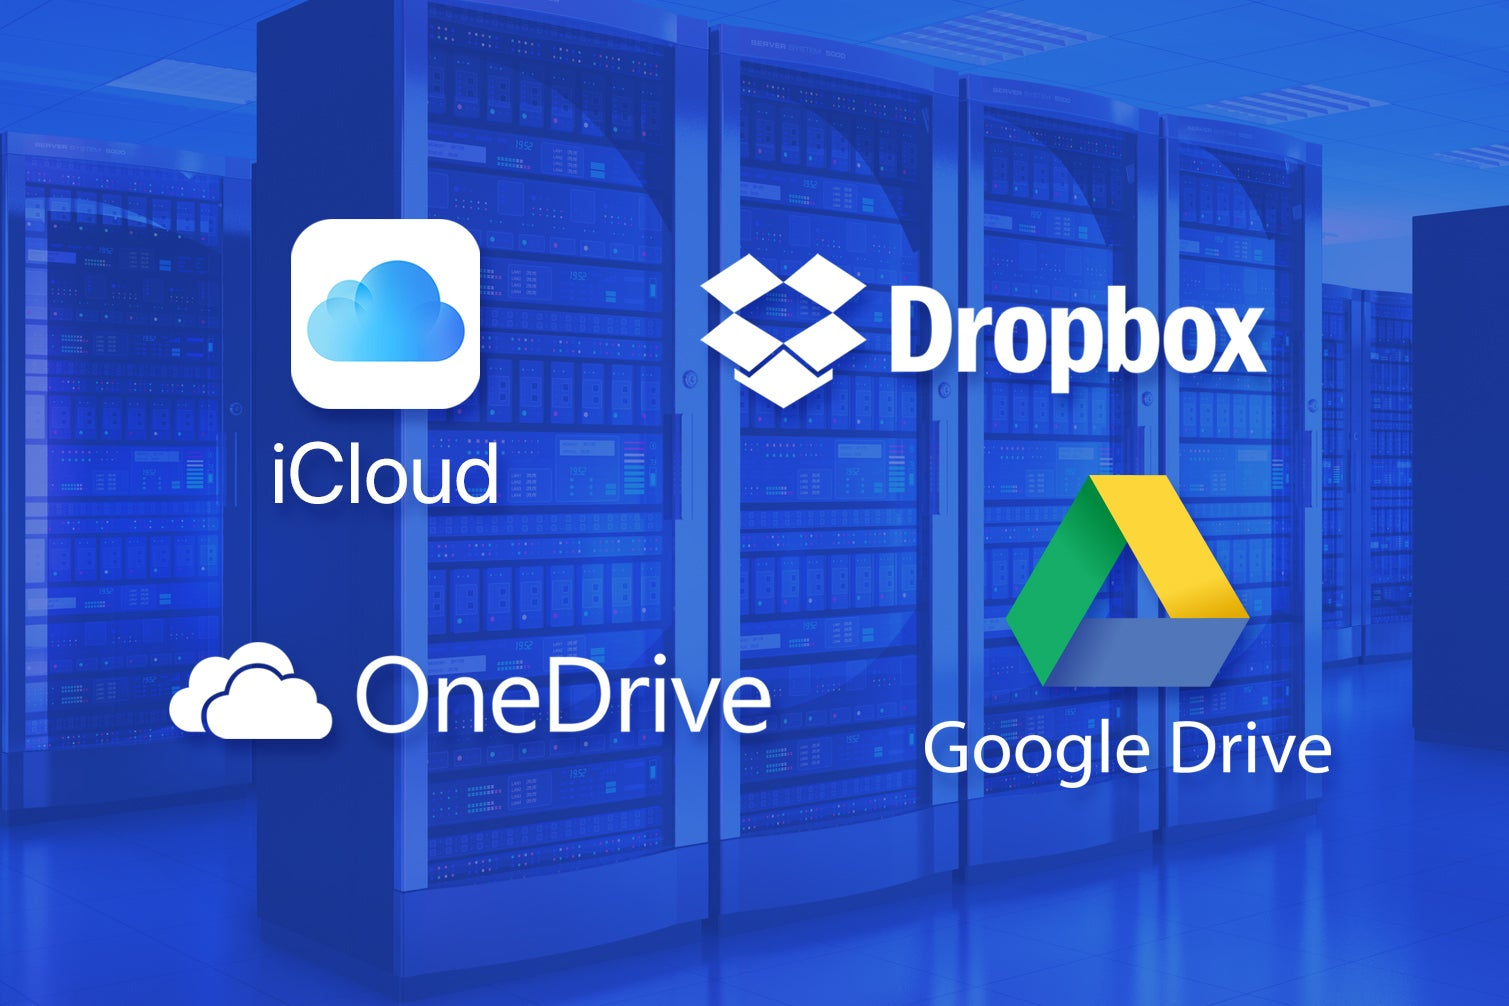
\includegraphics[height=3.5cm]{cloud-storage}
\end{center}

\section{\glsentrylong{NAS}}
\begin{itemize}
\item Data is stored in a \popup{specialized computer}{The computer
    rarely has a keyboard or monitor, and has many hard drive bays.}
  connected to the \gls{LAN}.
\item Usually mounts several \popup{disk}{Or disc.}s with some type of
  \gls{RAID} configuration.
\end{itemize}
\vspace{-4ex}
\begin{center}
  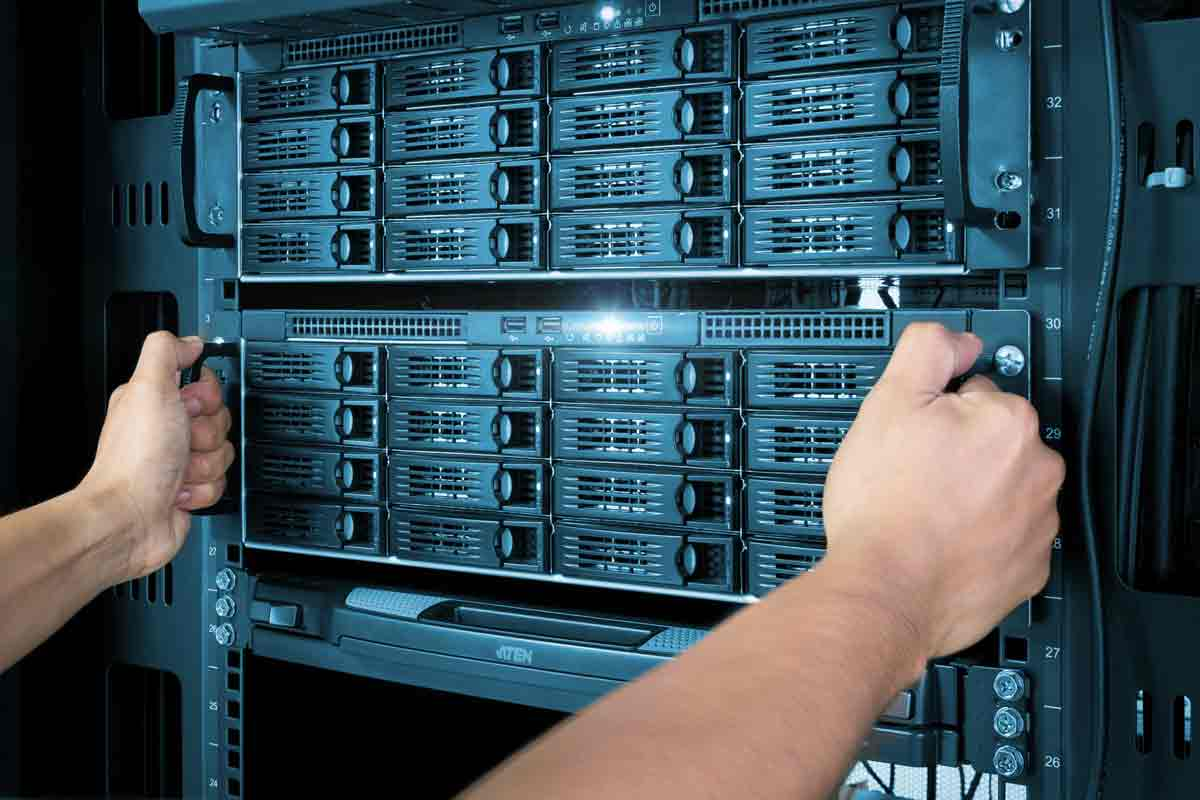
\includegraphics[height=3.5cm]{servidor-nas}
\end{center}

\section{\glsentrylong{RAID}}
\begin{itemize}
\item A \gls{RAID} is a logical disk that is able to work even when
  some of the \popup{physical disks}{That actually store the data.}
  fail. These are some of the existing configurations:
  \begin{enumerate}
  \item RAID-0 (Striping): \popup{No redundancy}{To maximize capacity,
      splits data across drives. This means that if a physical disk
      stops working, a loss of data will happen.}.
  \item RAID-1 (Mirroring): \popup{Maximum redundancy}{All physical
      disks contain the same data. To lost data all disks must fail at
      the same time.}.
  \item RAID-5 (Striping with Parity): \popup{One disk
      redundancy}{This configuration can only tolerate the failure of
      one disk.}. When the broken disk is replaced, the RAID must
    rebuild the parity information. During this time, no other disk
    can fail.
  \item RAID-6 (Double Parity): \popup{Two disks
      redundancy}{Tolerate the failure of
      two disks at the same time.}.
  \end{enumerate}
\end{itemize}

\section{\glsentrylong{HDD}}
\begin{itemize}
\item Electro-mechanical data storage-persistent device that uses
  magnetic storage to store and retrieve digital information.
\end{itemize}
\vspace{-4ex}
\begin{center}
  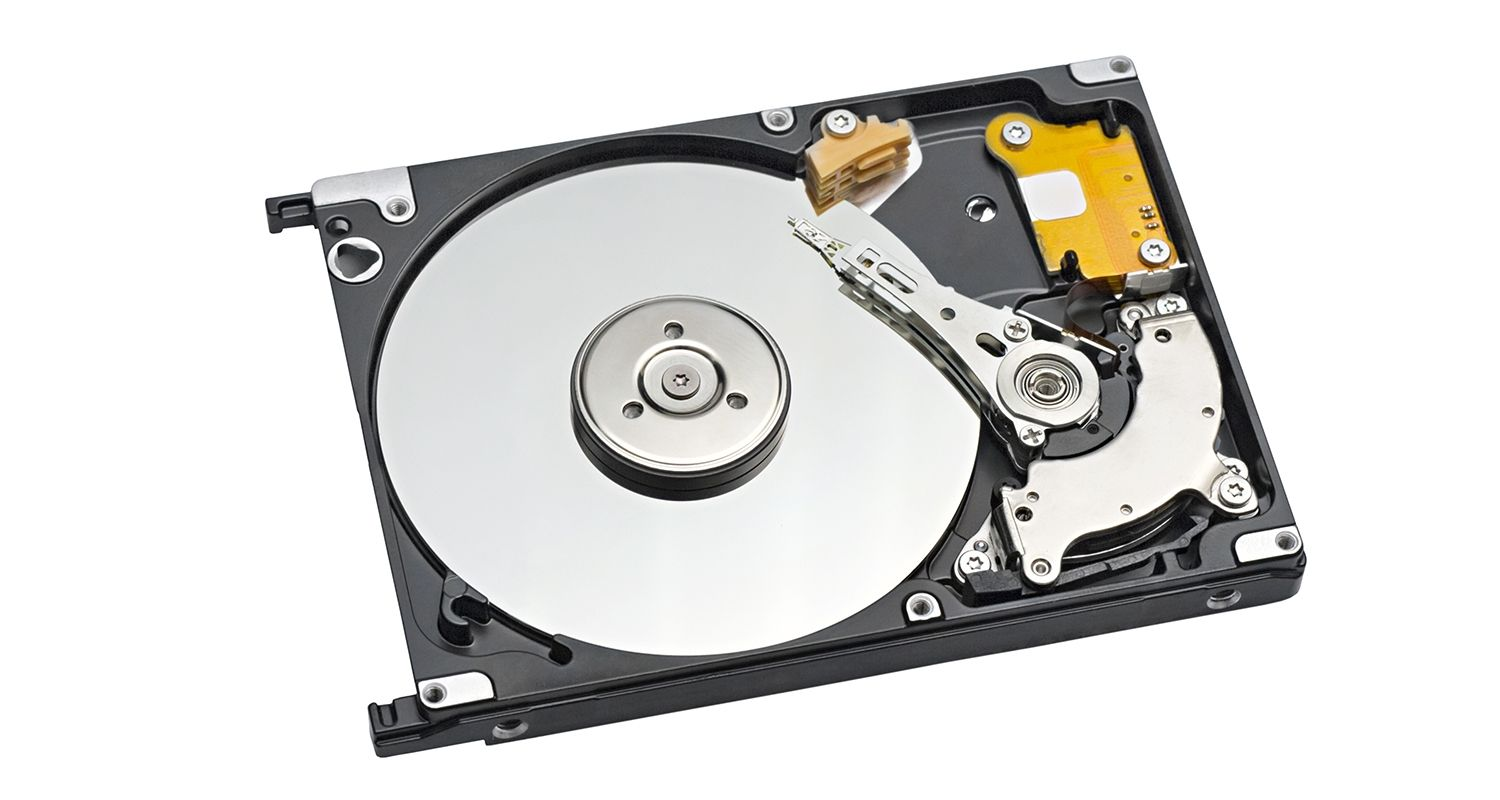
\includegraphics[height=3.5cm]{HDD}
\end{center}

\section{\glsentrylong{SSD}}
\begin{itemize}
\item Fully electronic storage device based on \popup{flash
    memory}{Flash memory is a type of non-volatile computer memory
    that can be electrically erased and reprogrammed. Unlike volatile
    memory (like RAM), it retains data even when the power is turned
    off.} chips.
\item Compared to \gls{HDD}s, \gls{SSD}s are faster, more reliable and
  power efficient, but for the same capacity, \gls{SSD}s are more
  expensive.
\end{itemize}
\vspace{-4ex}
\begin{center}
  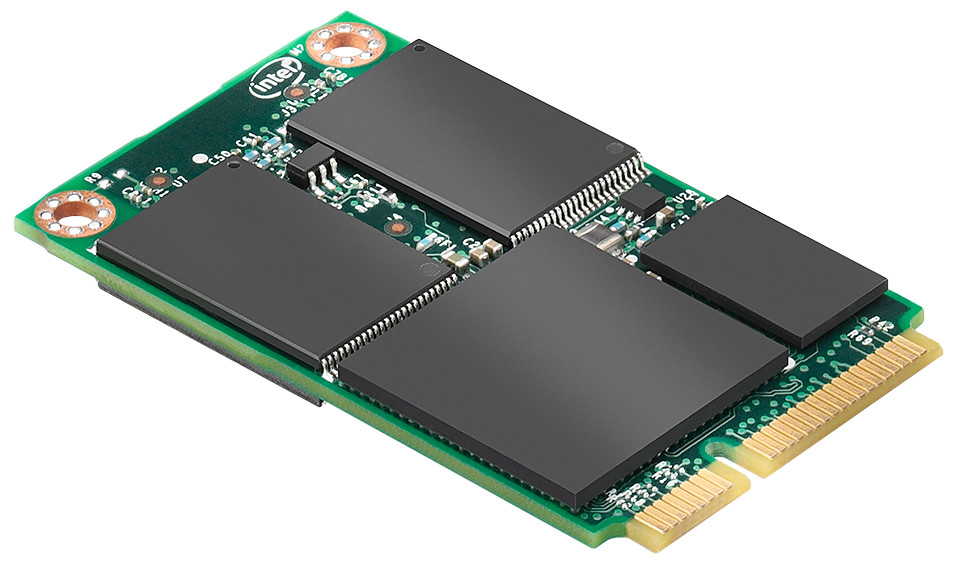
\includegraphics[height=3.5cm]{SSD}
\end{center}

\section{\glsentrylong{CD-ROM}}
\begin{itemize}
\item Optical storage medium that uses a laser to read digital data
  encoded on a spinning disc.
\item The data is stored as a spiral track of microscopic depressions
  genearted on a reflective aluminum layer encased in plastic.
\item Typical capacity: 800 GB.
\end{itemize}
\vspace{-4ex}
\begin{center}
  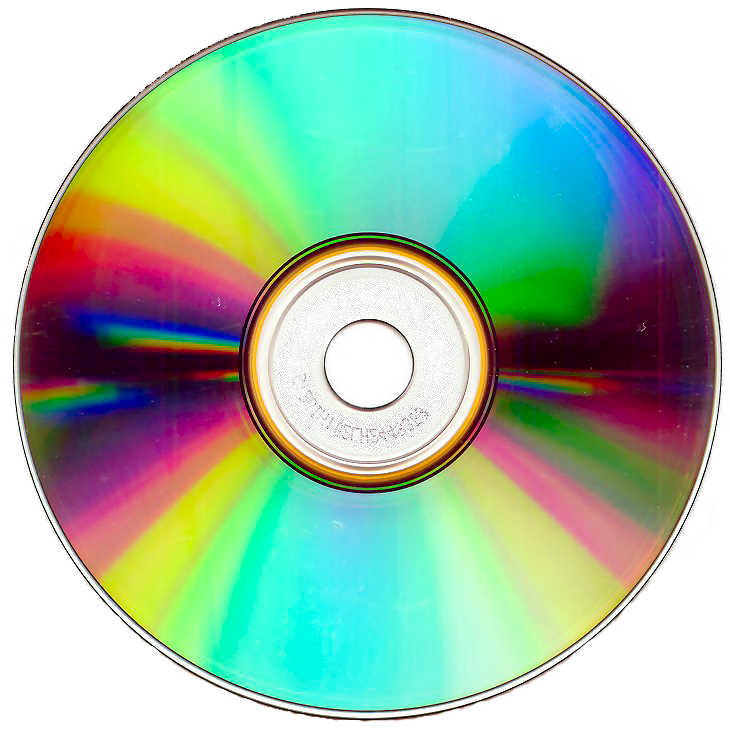
\includegraphics[height=3.5cm]{CD-ROM}
\end{center}
  
\section{\glsentrylong{CD-R}}
\begin{itemize}
\item A \gls{CD} that can be written once.
\end{itemize}
\vspace{-4ex}
\begin{center}
  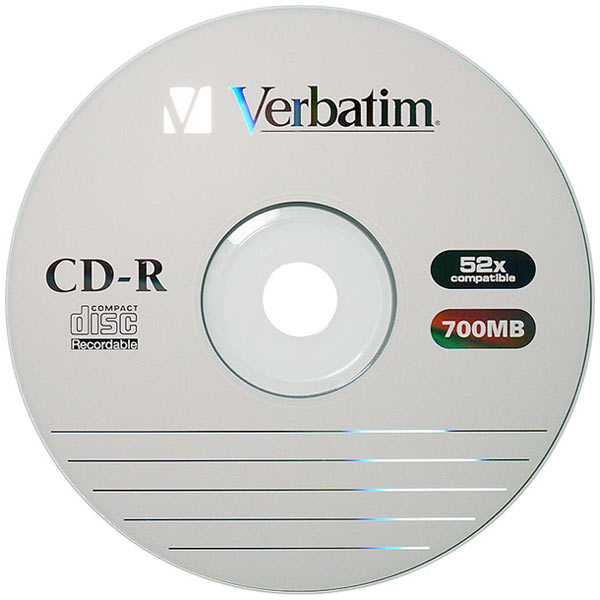
\includegraphics[height=3.5cm]{CD-R}
\end{center}

\section{\glsentrylong{CD-RW}}
\begin{itemize}
\item A \gls{CD} that can be written several times.
\end{itemize}
\vspace{-4ex}
\begin{center}
  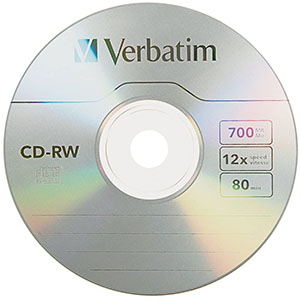
\includegraphics[height=3.5cm]{CD-RW}
\end{center}

\section{\glsentrylong{DVD}}
\begin{itemize}
\item The same than a \gls{CD-ROM} but with a higher capacity.
\item Typical capacity: 4.7 GB.
\item As with \gls{CD}, there are -R and -RW versions.
\end{itemize}
\vspace{-4ex}
\begin{center}
  
\includegraphics[height=3.5cm]{DVD-ROM}
\end{center}

\section{Blu-Ray}
\begin{itemize}
\item The same than a \gls{DVD-ROM} but with a higher capacity.
\item Typical capacity: Up to 100 GB.
\item As with \gls{DVD}, there are -R and -RW versions.
\end{itemize}
\vspace{-4ex}
\begin{center}
  
\includegraphics[height=3.5cm]{Blu-ray}
\end{center}

\section{Files and streams}
\begin{itemize}
\item A \popup{file}{Also known as ''archive''.} is a collection of data \popup{stored}{Files are
persistent: once written, they stay there until deleted.} on a storage
medium (for example, a NAS) with a defined structure and a
name. Example: a DICOM file.
\item A stream is a continuous flow of data that is transmitted and
processed in real-time, often without being stored
permanently. Example: a videcon between a patient and a doctor.
\item Files can be \popup{accesed randomly}{We can move over the file
to read or modify a part of it.}. Streams cannot (only are accesed
sequentially).
\end{itemize}

\section{Formats}
\begin{itemize}
\item Files and streams must follow some predefined structure and
encodings that indicate how to recover the information contained.
\item Most of the image formats used in medicine follow some standard
which define they, such as for example, the DICOM format.
\end{itemize}

\section{Data compression}
\begin{itemize}
\item Images requires large amounts of data to be represented. Data
compression define the objective of an efficient encoding system:
reduce the lendth of files and streams.
\item Data compressors can be:
\begin{enumerate}
\item \textbf{Lossless}: If after the decompression we recover all the
compressed information, to the point that the original file/stream can
be regenerated.
\item \textbf{Lossy}: when not. The advantage is that the compression
ratios are much higher, and sometimes the loss can be aceptable.
\end{enumerate}
\end{itemize}

\section{Long-term persistency, data sequrity and privacy}
\begin{itemize}
\item Medical images contain important information and should be
  stored in long-term persistence storage systems.
\item Patient images are protected health information. Therefore,
  \gls{PACS} must follow laws like HIPAA (USA) or GDPR (Europe) for
  confidentiality.
\item Medical images should only be accessed by authorized healthcare
  professionals.
\end{itemize}